%% Define the logo at the bottom right corner
%\logo{\includegraphics[height=0.7cm]{fig/inr_logo_cherch_UK_coul}}

\begin{frame}
    \titlepage
\end{frame}
\note{
}

% Reset the logo: for all following slides, logo is substituted by page number
\setbeamercolor*{logo}{fg=black}
\logo{\insertframenumber}
%\logo{\insertframenumber/\inserttotalframenumber}

%%%%%%%%%%%%%%%%%%%%%%%%%%%%%%%%%%%%%%%%%%%%%%%%%%%%%%%%%%%%%%%%%%%%%%%%%%%%%%%

\section{Introduction}
\subsection{Introduction}

\begin{frame}{\mcts{} (MCTS)}
    \begin{itemize}
        \item MCTS is a recent algorithm for {\em sequential decision making}
        \item It applies to \mdp{} (MDP)
        \begin{itemize}
            \item discrete-time $t$ with finite horizon $\horizon$
            \item state $\state_t \in \statespace$
            \item action $\decision_t \in \decisionspace$
            \item transition function $\state_{t+1} = \transitionfunction(\state_t, \decision_t)$
            \item cost function $\reward_t = \costfunction_\transitionfunction(\state_t)$
            \item reward $\globalreward = \sum_{t = 0}^{\horizon}{\reward_t}$
            \item policy function $\decision_t = \policy_{\transitionfunction}(\state_t)$
            \item we look for the policy $\policy^*$ that maximizes expected $\globalreward$ 
        \end{itemize}
    \end{itemize}
\end{frame}


\begin{frame}{MCTS strength}
    \begin{itemize}
        \item Mcts is a versatile algorithm (it does not require knowledge about the problem)
        \item especially, does not require any knowledge about the Bellman value function
        \item stable on high dimensional problems
        \item it outperforms all other algorithms on some problems (difficult games like Go, general game playing, \dots)
    \end{itemize}
\end{frame}


\begin{frame}{MCTS}
    Problems are represented as a tree structure:
    \begin{itemize}
        \item blue circles = states
        \item plain edges + red squares = decisions
        \item dashed edges = stochastic transitions between two states
    \end{itemize}
    \begin{center}
        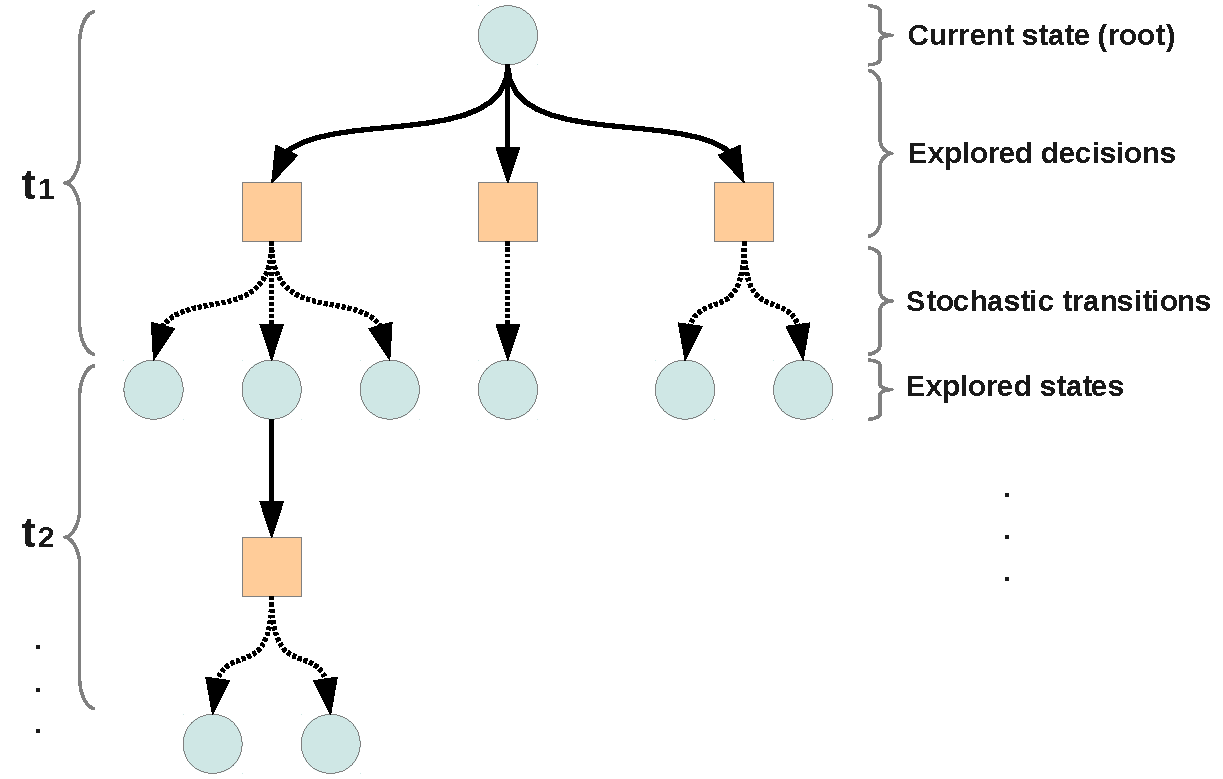
\includegraphics[width=.65\linewidth]{figs/tree}
    \end{center}
\end{frame}


%\begin{frame}{Overview}
%    \tableofcontents[hideallsubsections]
%\end{frame}
%\note{
%}

%%%%%%%%%%%%%%%%%%%%%%%%%%%%%%%%%%%%%%%

\section{\mcts{}}
\subsection{\mcts}

\begin{frame}{Main steps of MCTS}
    \begin{center}
        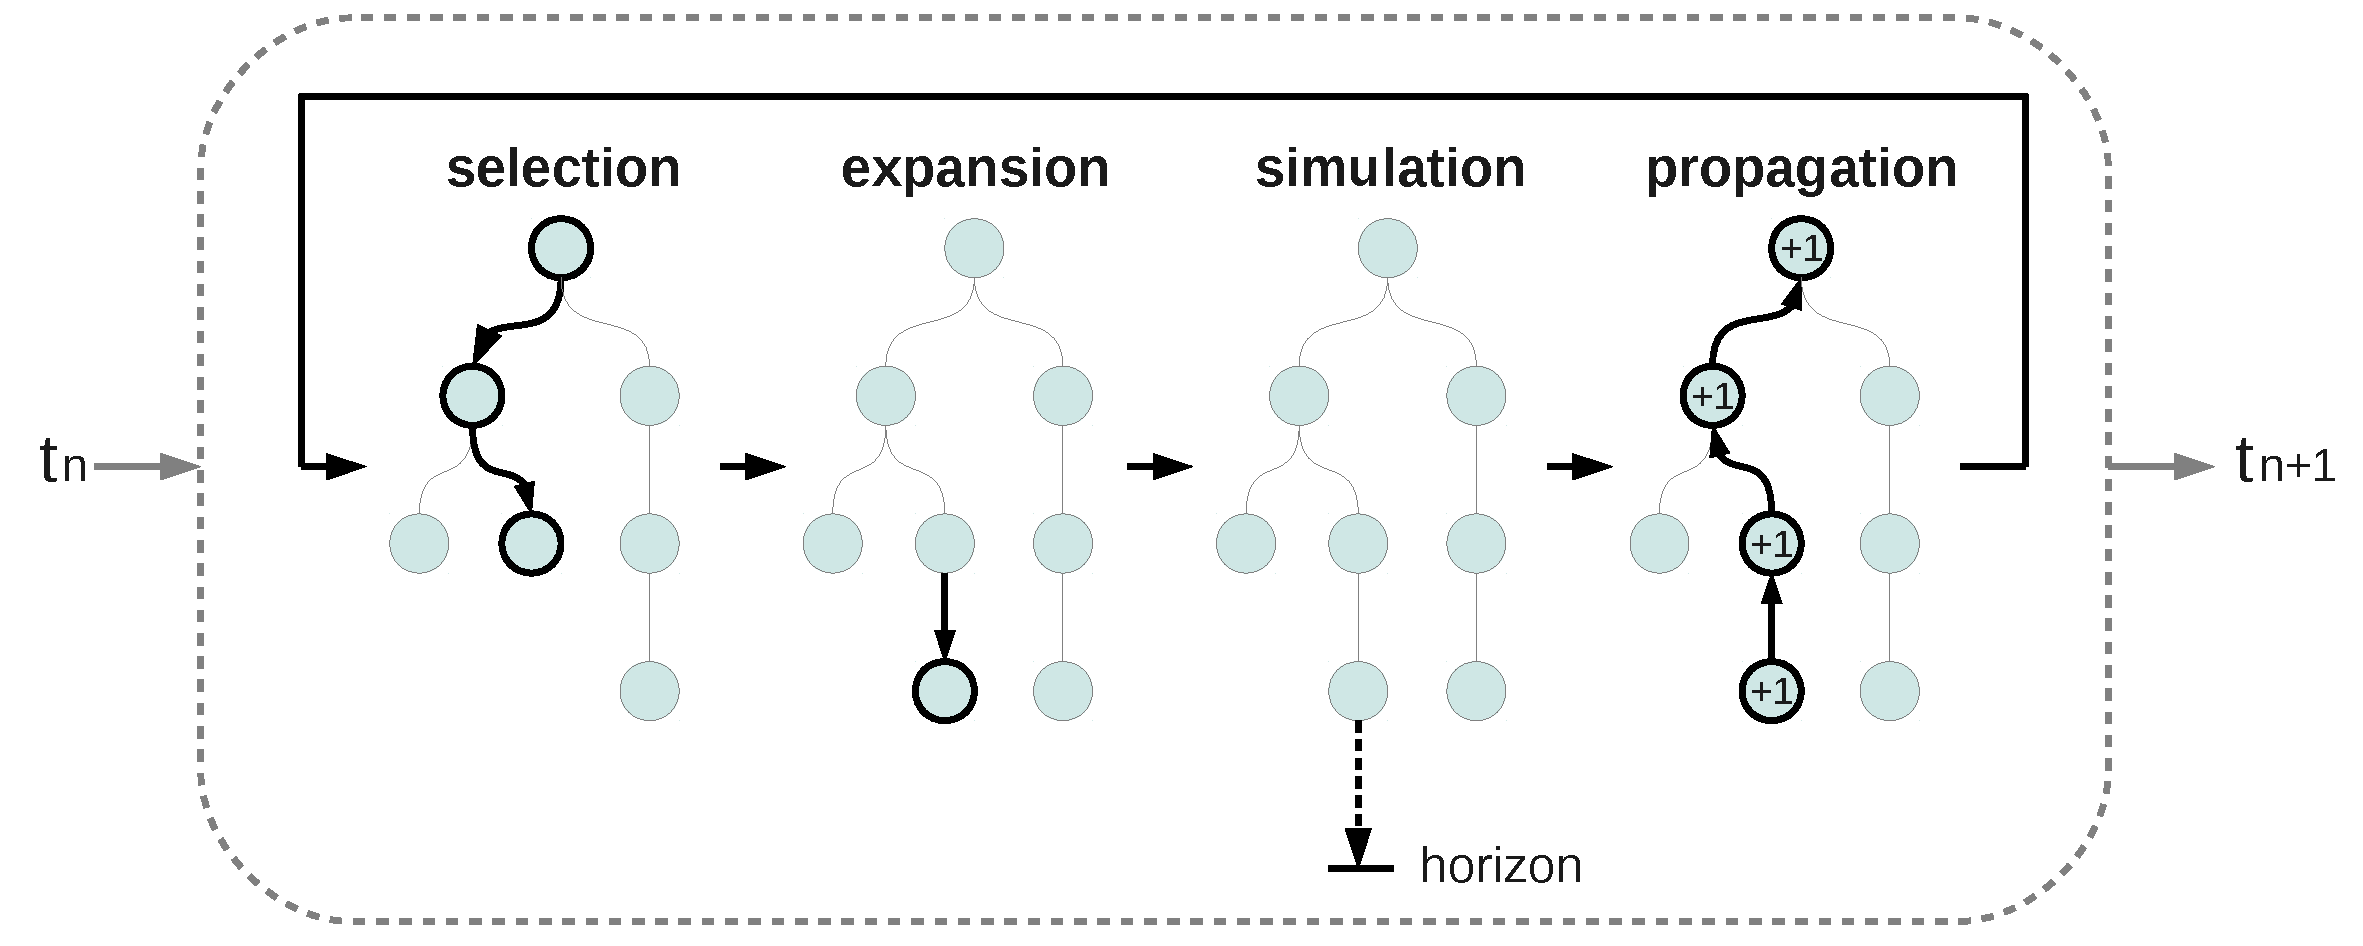
\includegraphics[width=.99\linewidth]{figs/tree9}
    \end{center}
\end{frame}


\begin{frame}{Main steps of MCTS}
    \only<1| handout:0> {
        \begin{center}
            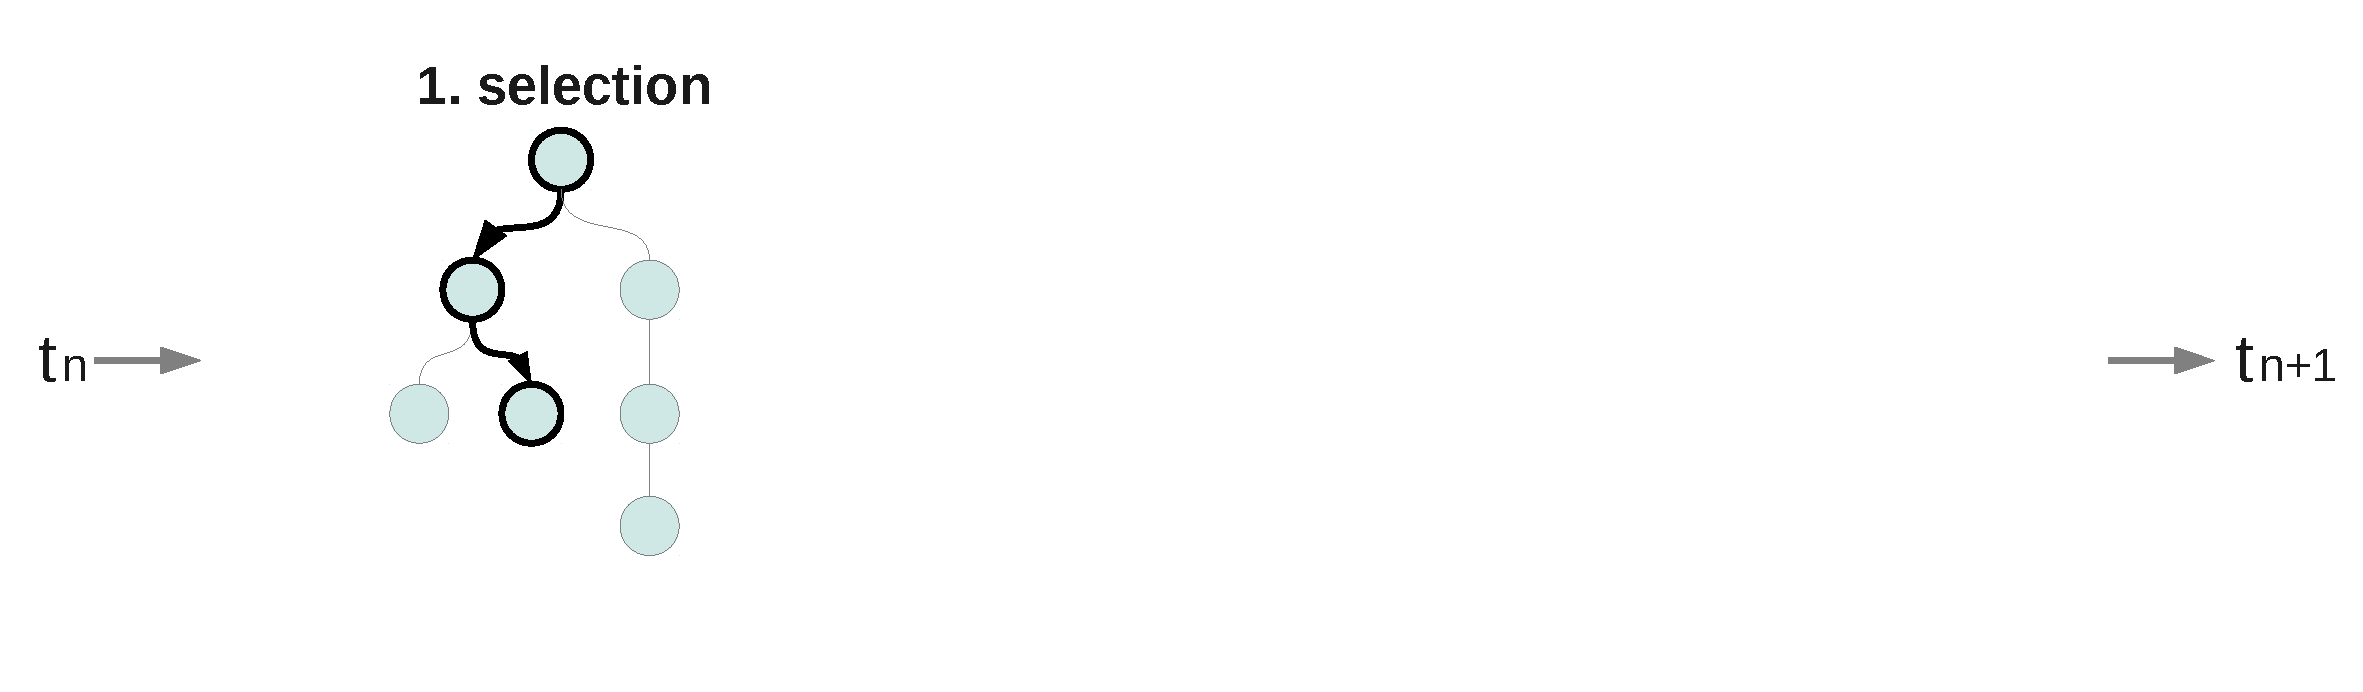
\includegraphics[width=.75\linewidth]{figs/tree10a}
        \end{center}
    }
    \only<2| handout:0> {
        \begin{center}
            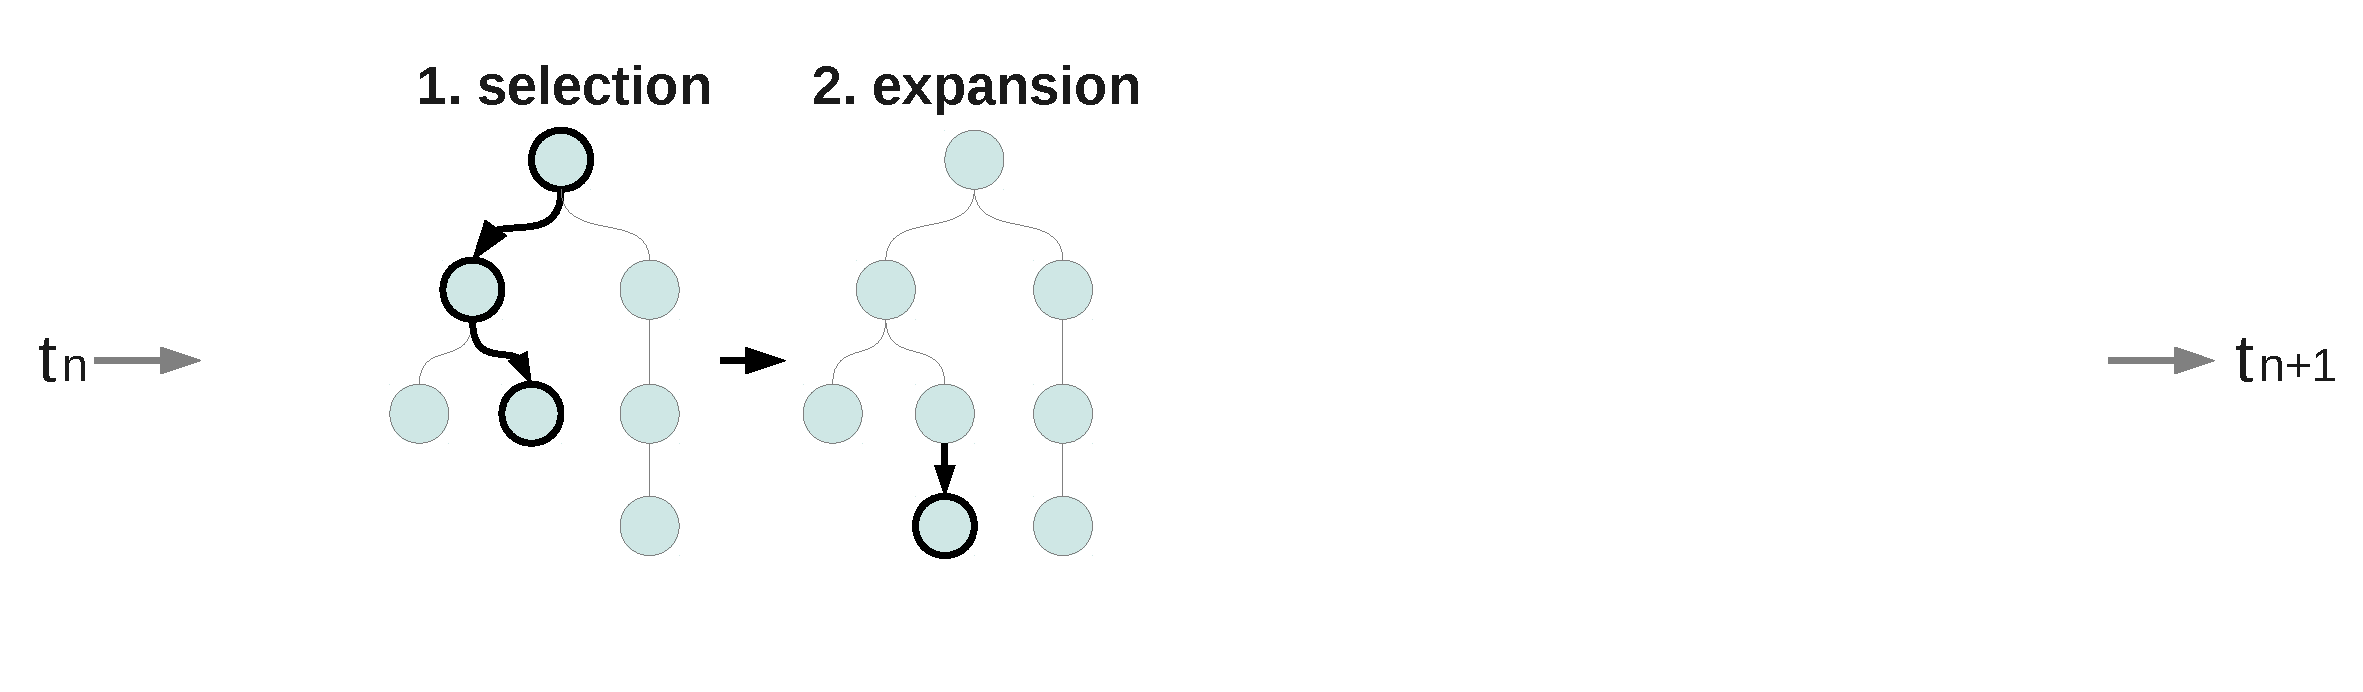
\includegraphics[width=.75\linewidth]{figs/tree10b}
        \end{center}
    }
    \only<3| handout:0> {
        \begin{center}
            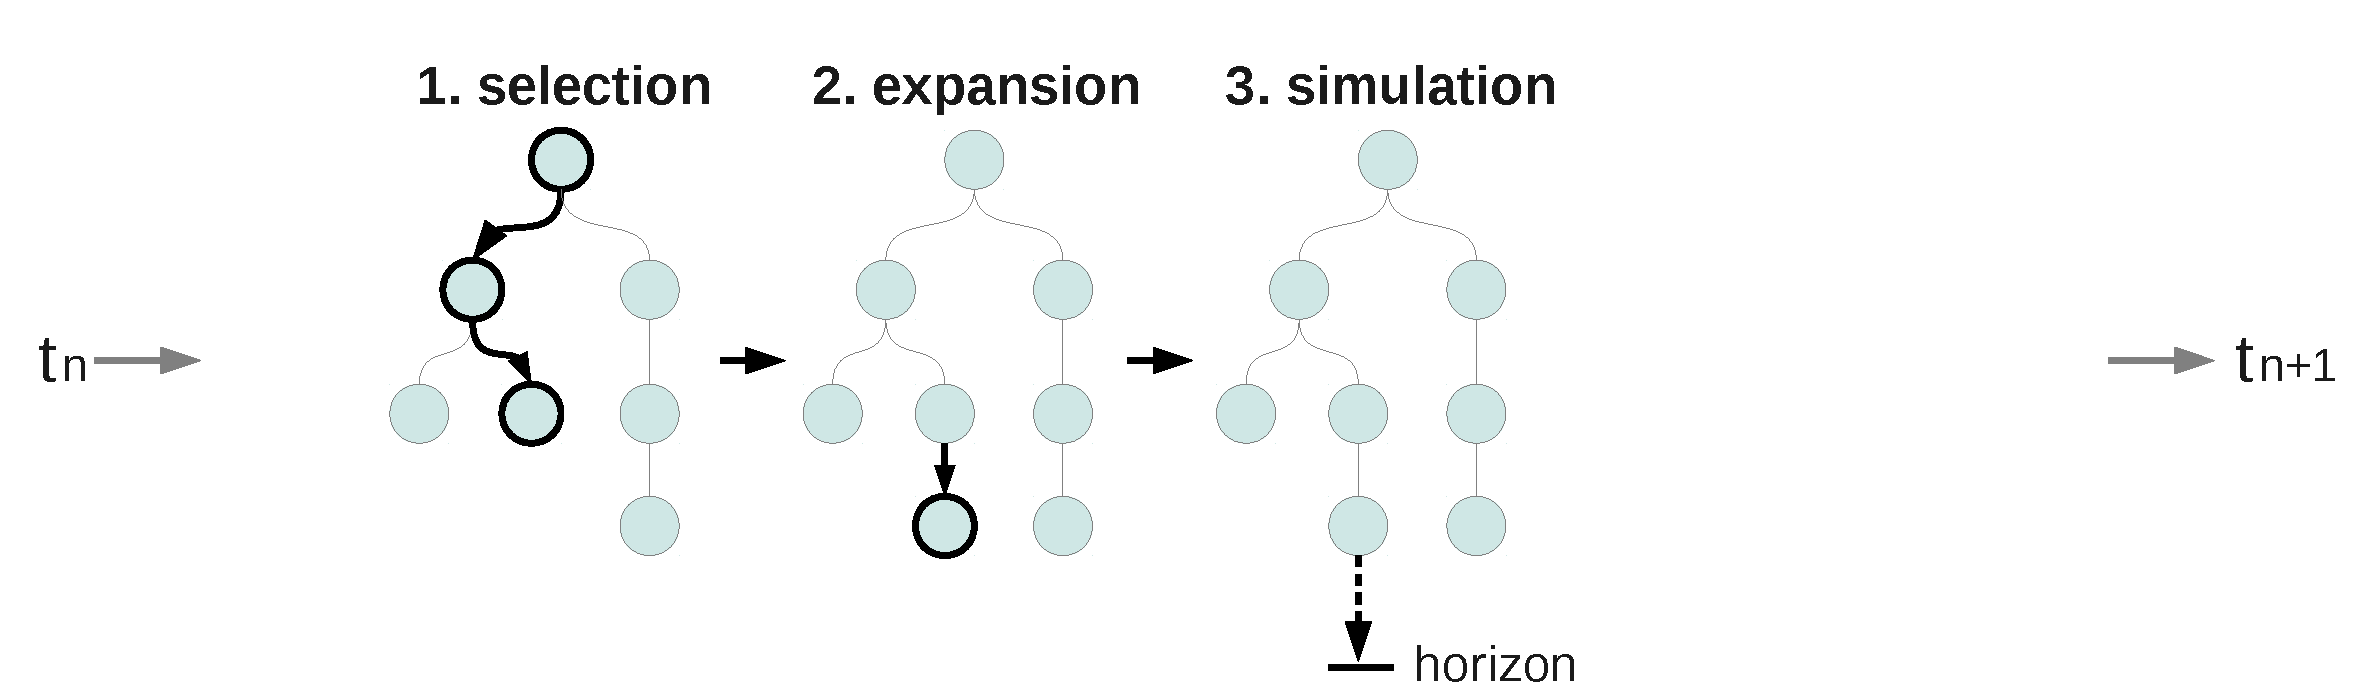
\includegraphics[width=.75\linewidth]{figs/tree10c}
        \end{center}
    }
    \only<4| handout:0> {
        \begin{center}
            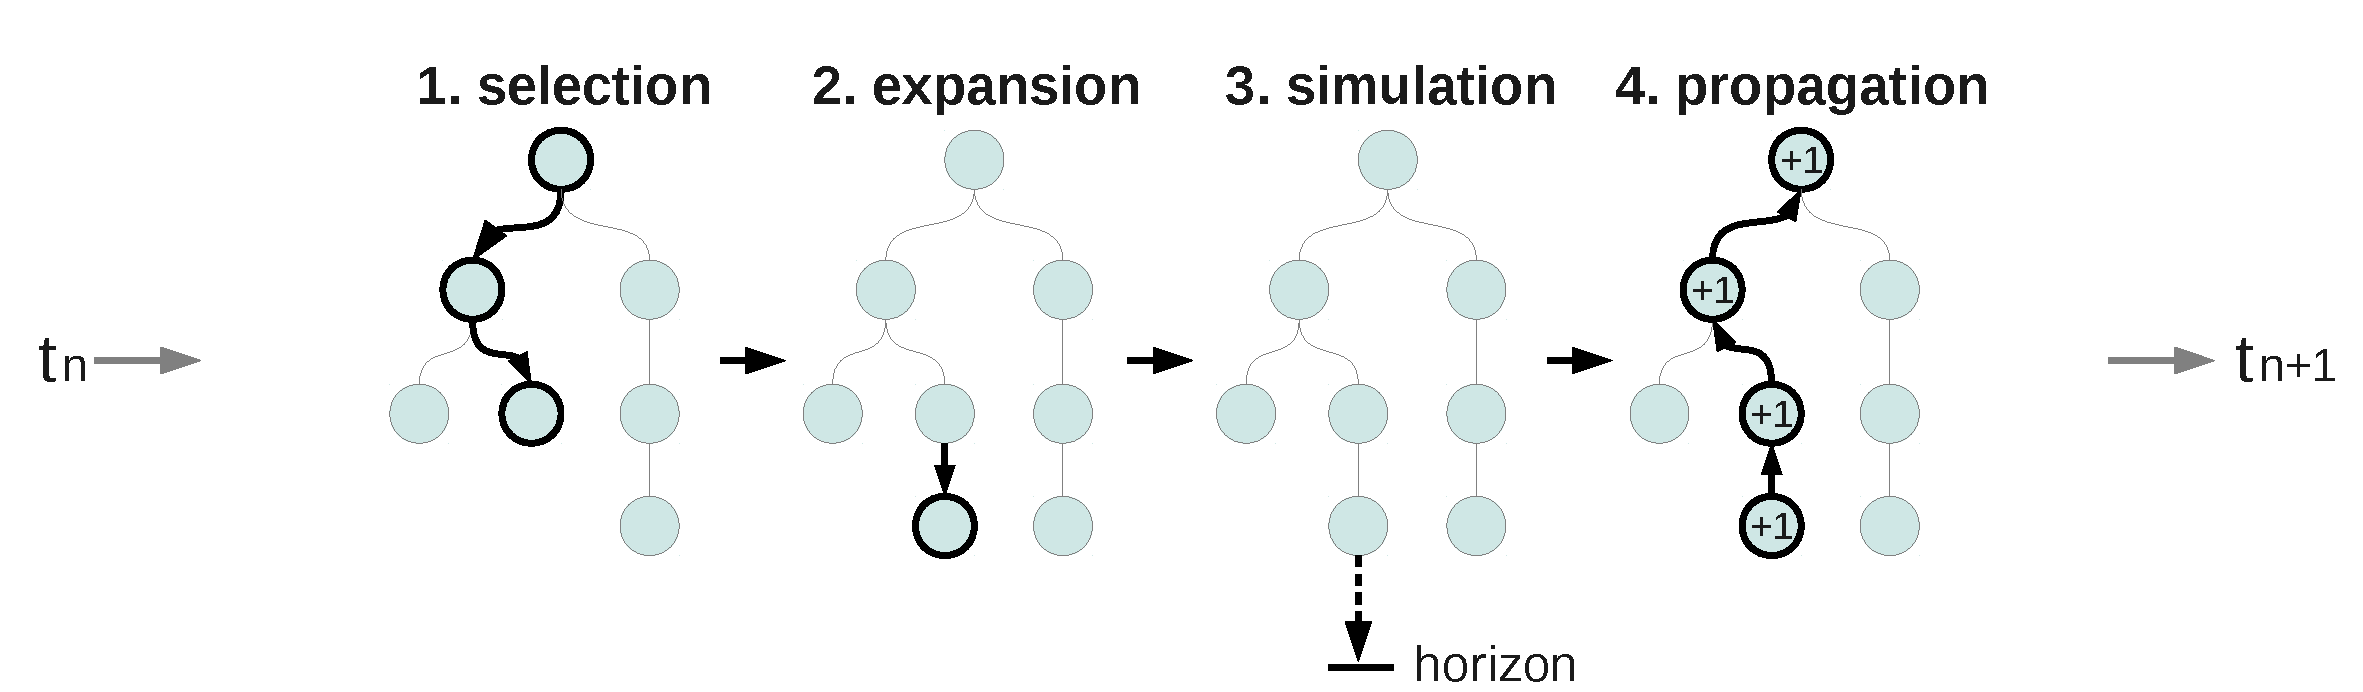
\includegraphics[width=.75\linewidth]{figs/tree10d}
        \end{center}
    }
    \only<5> {
        \begin{center}
            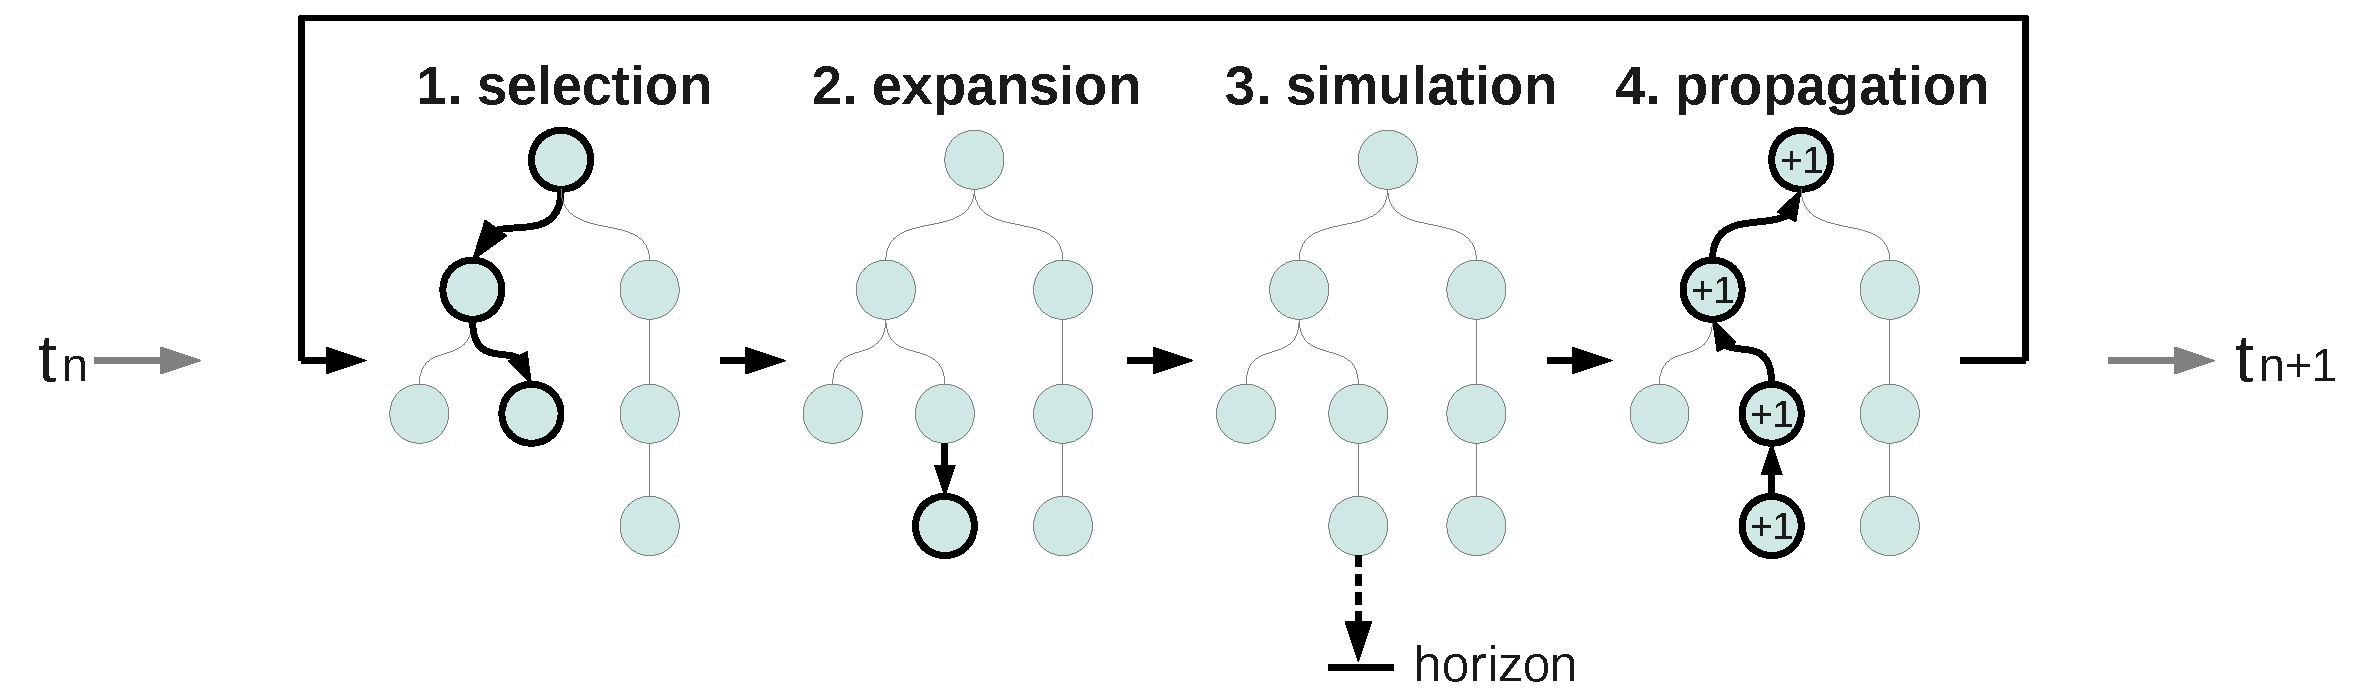
\includegraphics[width=.75\linewidth]{figs/tree10e}
        \end{center}
    }
    \begin{small}
        Starting from an initial state:%, repeat next steps until time budget is over:
        \begin{enumerate}
            \item<1-> select the state we want to expand from
            \item<2-> add the generated state in memory
            \item<3-> evaluate the new state with a default policy until horizon is reached
            \item<4-> back-propagation of some information:
            \begin{itemize}
                \item $n(\state,\decision)$ : number of times decision $\decision{}$ has been simulated in $\state$
                \item $n(\state)$ : number of time $\state$ has been visited in simulations
                \item $\hat{Q}(\state,\decision)$ : mean reward of simulations where $\decision$ was whosen in $\state$
            \end{itemize}
        \end{enumerate}
        ~\\
    \end{small}
\end{frame}


\begin{frame}{Main steps of MCTS}
    \begin{center}
        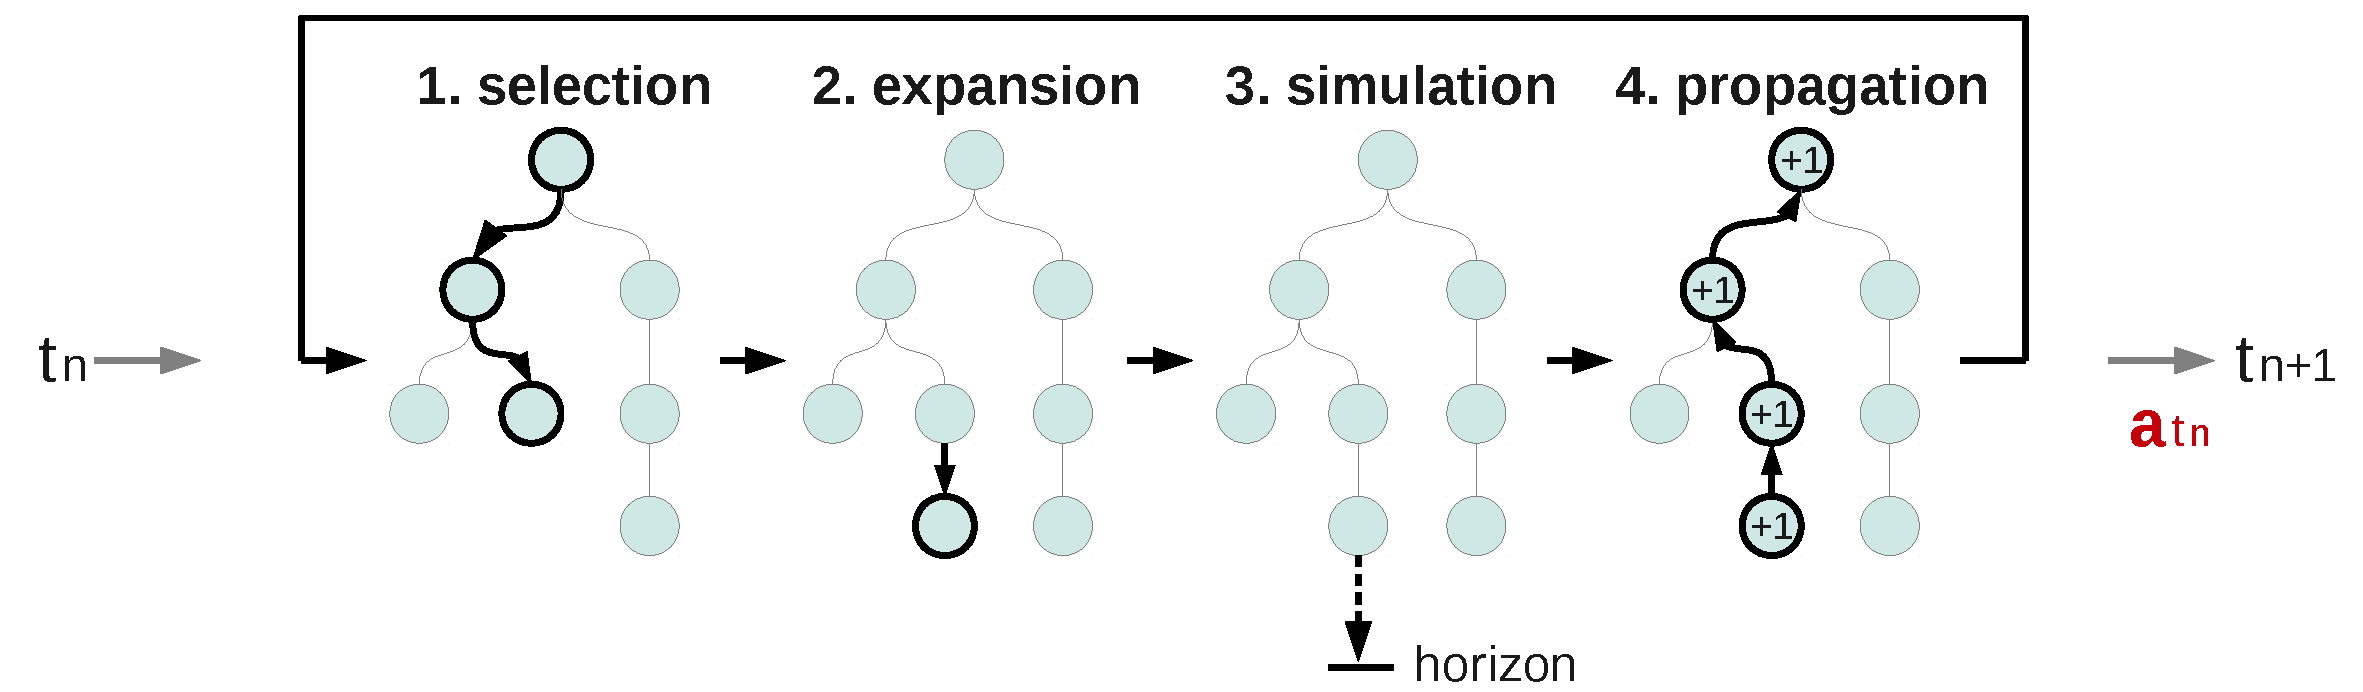
\includegraphics[width=.75\linewidth]{figs/tree10f}
    \end{center}

    \begin{block}{The selected decision}
        $\decision_{t_n}$ = the most visited decision form the current state (root node)
    \end{block}
\end{frame}


%%%%%%%%%%%%%%%%%%%%%%%%%%%%%%%%%%%%%%%

\section{Selection and expansion}
\subsection{Selection and expansion}

\begin{frame}{Selection step}
    How to select the state to expand~?
    \begin{center}
        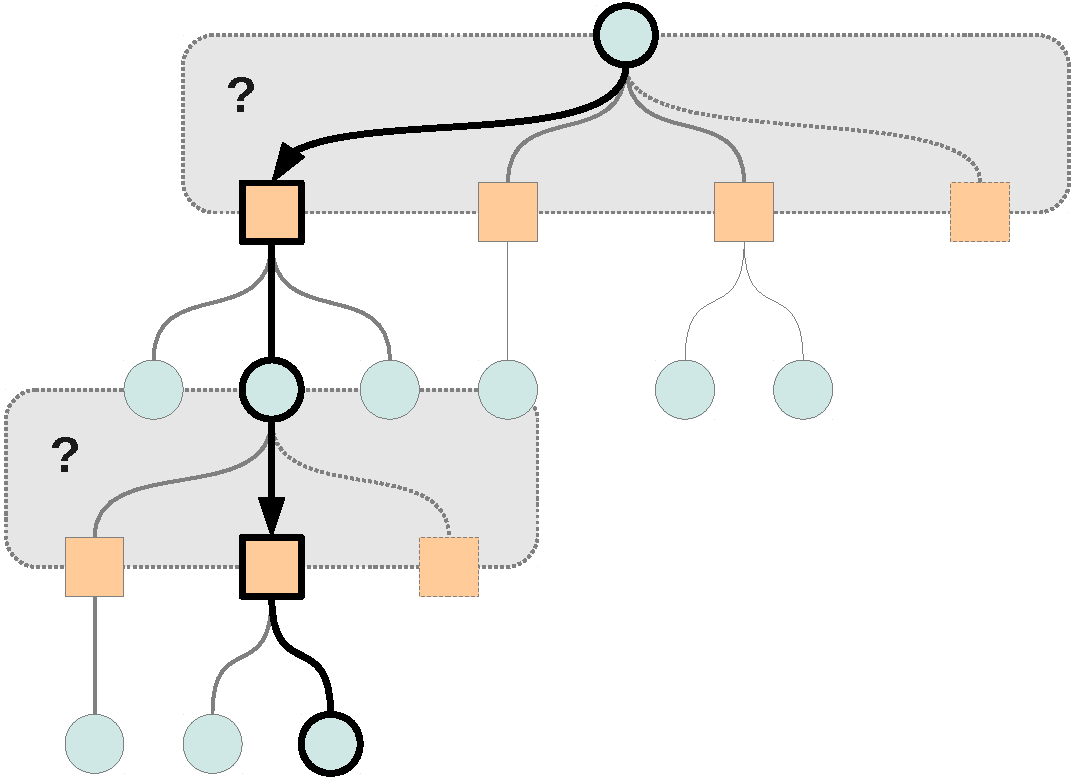
\includegraphics[width=.80\linewidth]{figs/tree3}
    \end{center}
\end{frame}


\begin{frame}{How to select the state to expand~?}
    \begin{center}
        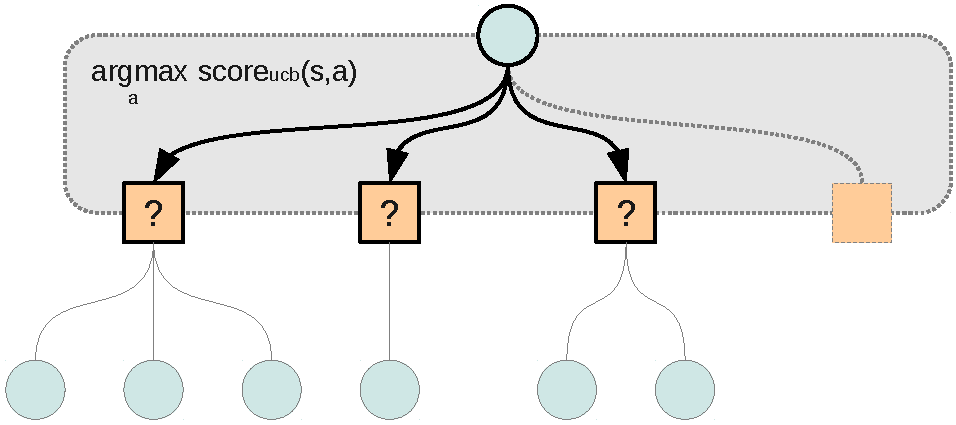
\includegraphics[width=.40\linewidth]{figs/tree4}
    \end{center}
    The {\em selection} phase is driven by \ucb{}% algorithm, knowing:
    $$
    %\scoreucb(\state, \decision) = \underbrace{\frac{1}{n_{\decision}} \sum_{0 \leq t \leq n_{\decision}}{\reward_t}}_\text{1} + K \underbrace{\sqrt{\frac{\log(N)}{n_{\decision}}}}_\text{2}
    \scoreucb(\state, \decision) = \underbrace{\hat{Q}(\state,\decision)}_\text{1} + \underbrace{\sqrt{ \frac{\log(2 + n(\state))}{2 + n(\state, \decision)} }}_\text{2}
    $$
    \only<1| handout:1> {
        \begin{enumerate}
            %\item the average reward of known actions
            \item mean reward of simulations including action $\decision$ in state $\state$
            \item the uncertainty on this estimation of the action’s value
        \end{enumerate}
    }
    \only<2| handout:2> {
        The selected action: $$\decision^\star = \arg\max_{\decision} ~ \scoreucb(\state, \decision)$$
        ~\\
    }
    ~\\
\end{frame}


\begin{frame}{How to select the state to expand~?}
    \begin{center}
        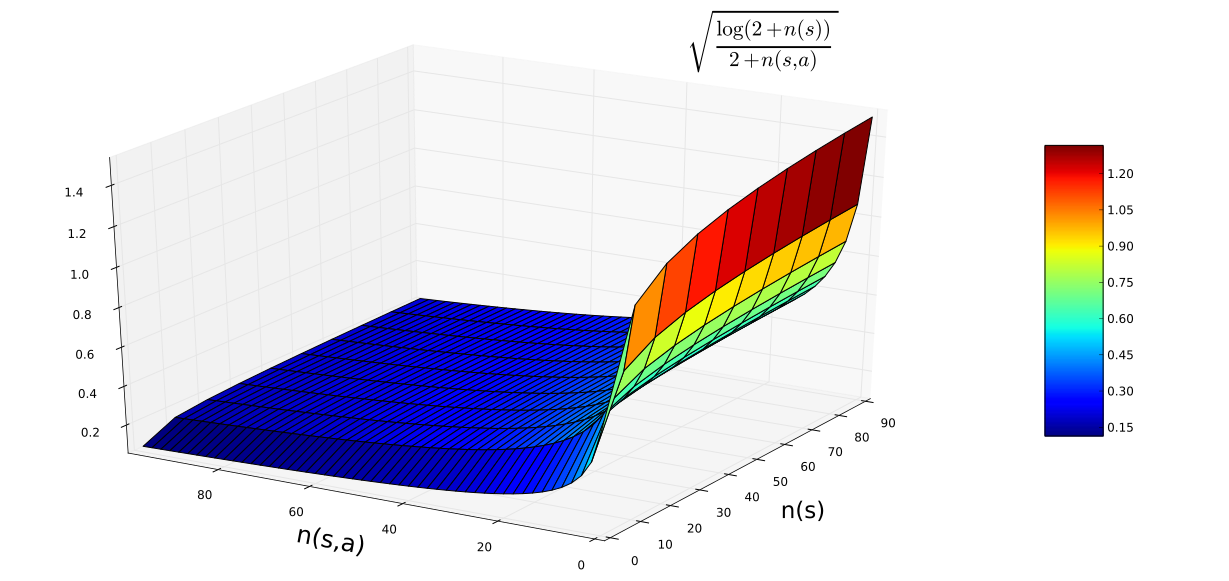
\includegraphics[width=.90\linewidth]{figs/ucb_func2}
    \end{center}
\end{frame}


\begin{frame}{When should we expand?}
    \begin{center}
        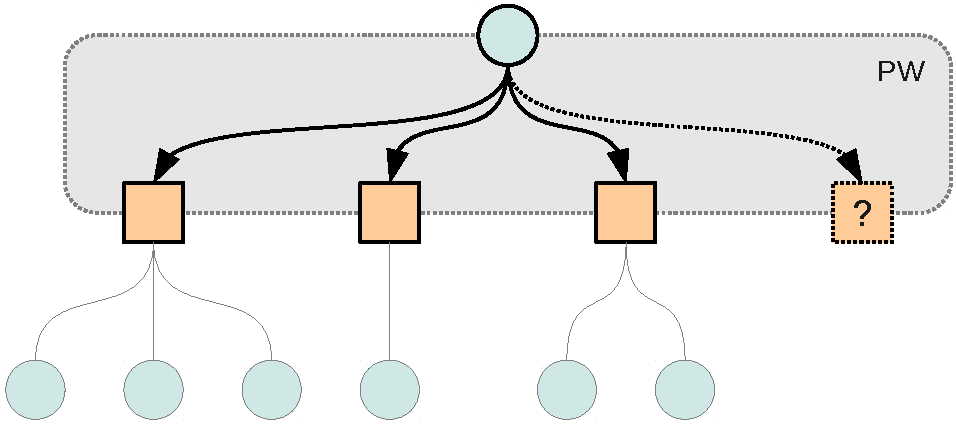
\includegraphics[width=.40\linewidth]{figs/tree5}
    \end{center}

    One standard way of tackling the exploration/exploitation dilemma
    is \pw.\\
    ~\\
    A new parameter $\alpha \in [0 ; 1]$ is introduced, to choose between exploration (add a decision to
    the tree) and exploitation (go to an existing node)
\end{frame}


\begin{frame}{How to select the state to expand~?}
    \begin{center}
        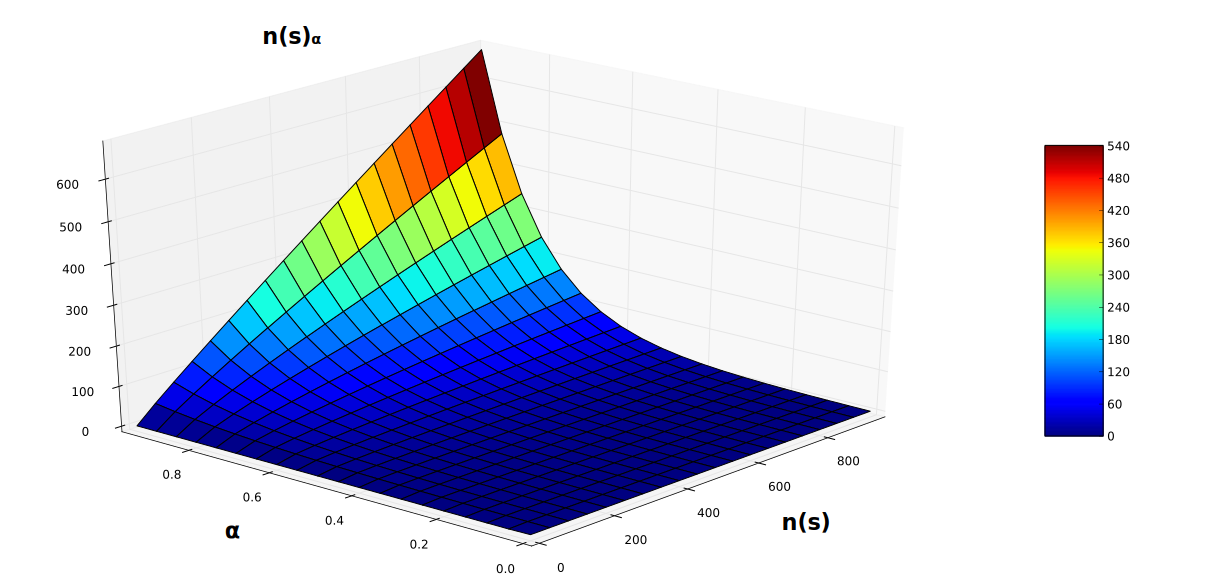
\includegraphics[width=.80\linewidth]{figs/pw_func}
    \end{center}

    \begin{itemize}
        \item $\text{if}( |\subdecisionspace{}_{\state}| < n(\state)^{\alpha} )$ then we explore a new decision
        \item else we simulate a known decision
    \end{itemize}

    With $|\subdecisionspace{}_{\state}|$ the number of legal actions in state $\state$\\
    ~\\
\end{frame}


\begin{frame}{When should we expand?}
    $\alpha = 0.2$
    \begin{center}
        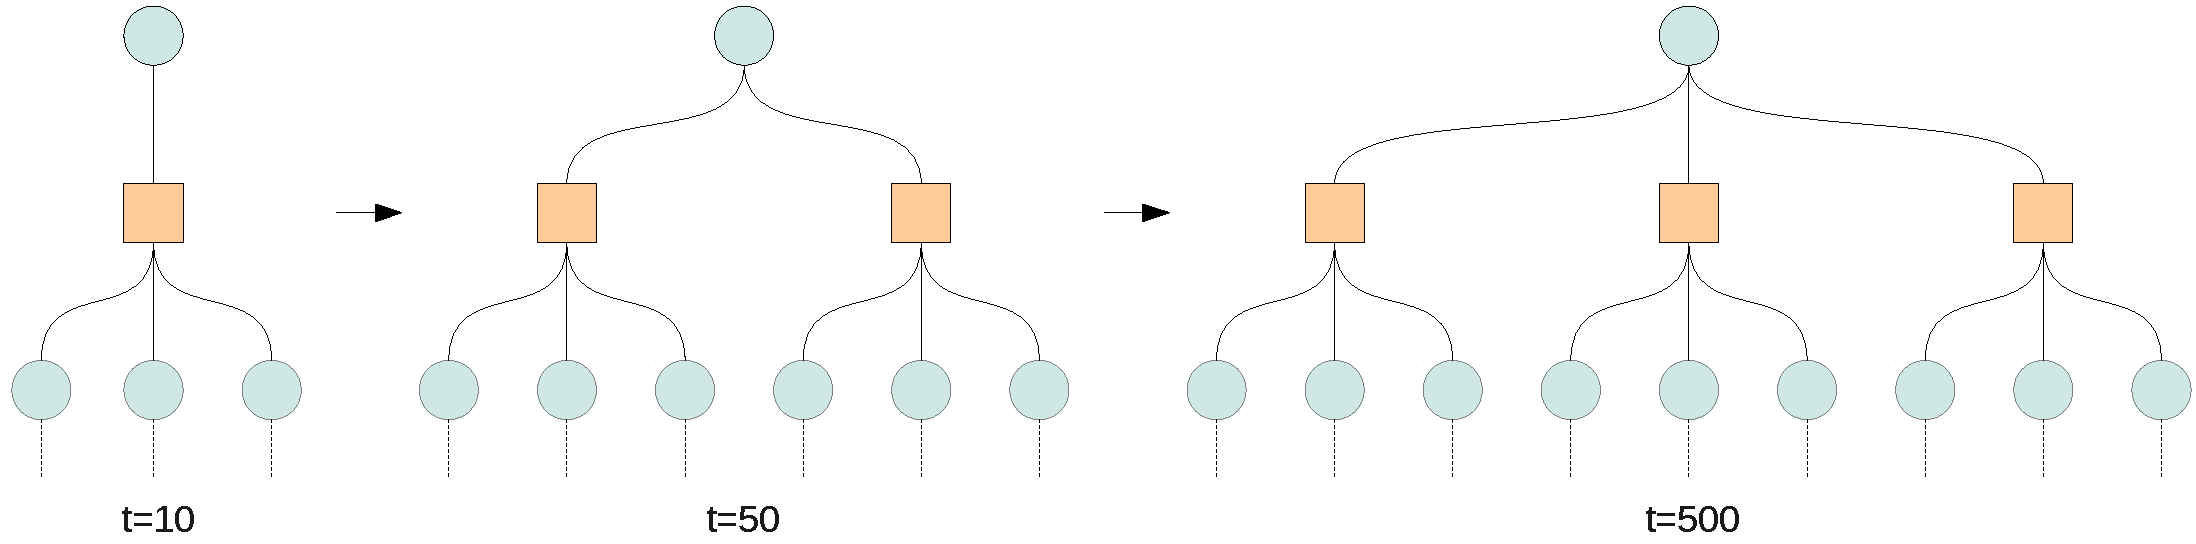
\includegraphics[width=.70\linewidth]{figs/tree6}
    \end{center}

    $\alpha = 0.8$
    \begin{center}
        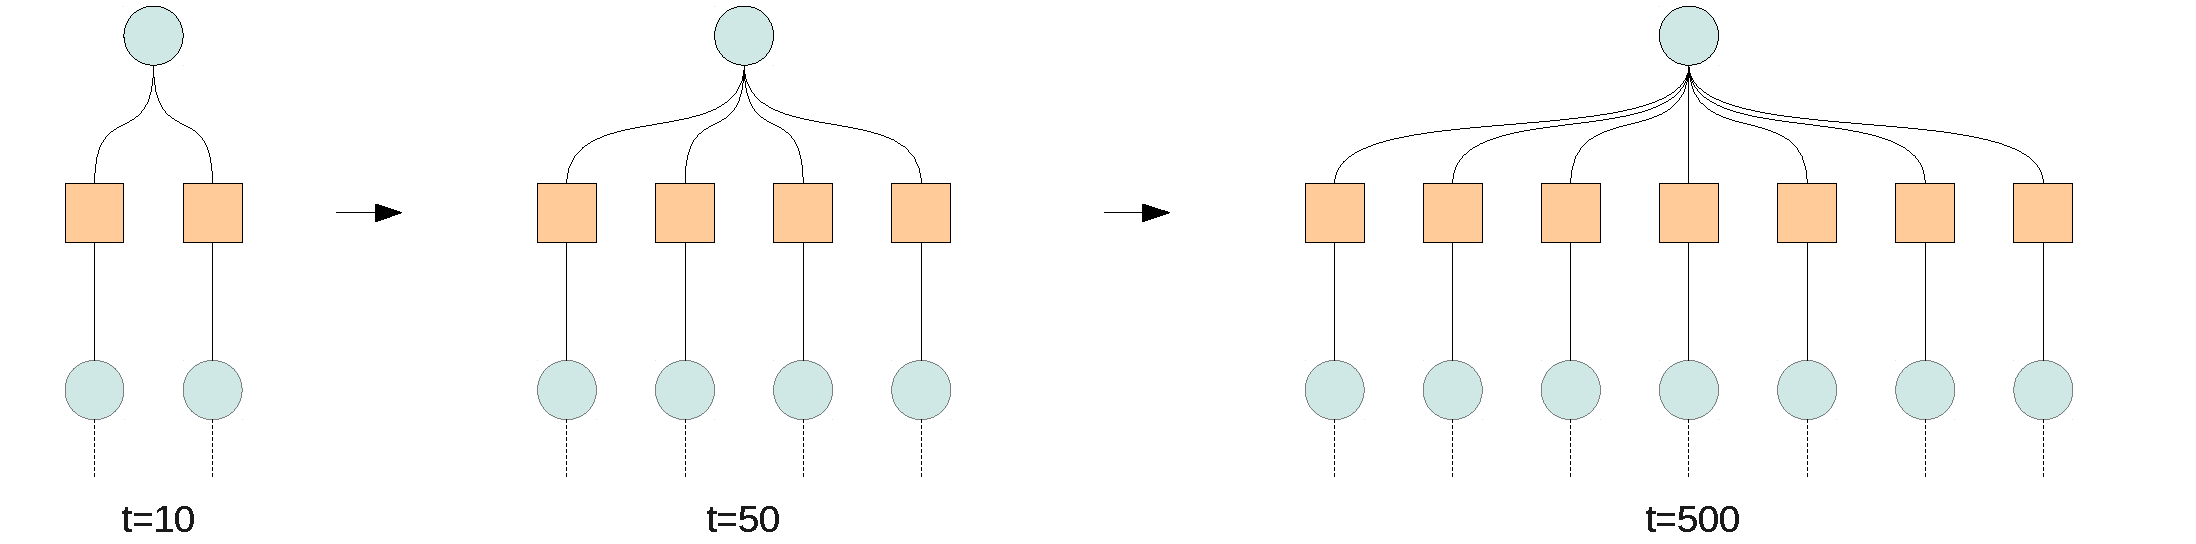
\includegraphics[width=.70\linewidth]{figs/tree7b}
    \end{center}
\end{frame}


%%%%%%%%%%%%%%%%%%%%%%%%%%%%%%%%%%%%%%%%%%%%%%%%%%%%%%%%%%%%%%%%%%%%%%%%%%%%%%%

%\section{Conclusion}

%%%%%%%%%%%%%%%%%%%%%%%%%%%%%%%%%%%%%%%%%%%%%%%%%%%%%%%%%%%%%%%%%%%%%%%%%%%%%%%%

\subsection{Conclusion}

\begin{frame}{TODO}{TODO}
    
    TODO

\end{frame}
\note{
}


%\begin{frame}{Thank you for your attention}
%    \begin{center}
%        Questions ?
%    \end{center}
%\end{frame}
%\note{
%}

%\section*{Bibliography}
\section*{References}

\begin{frame}[allowframebreaks]
    \frametitle{References}

    %\nocite{TEST14}  % fait apparaitre le document dans la bibliographie sans le citer !
    \nocite{*}        % fait apparaitre TOUS les documents du .bib dans la bibliographie sans les citer !

    \bibliographystyle{amsalpha} % name of the .bst file (bibliography style)
    \bibliography{bibliography}  % name of the .bib file (without the file name extension)
\end{frame}
\note{
}

%\appendix

\section{Appendix}

\begin{frame}{Title}{Subtitle}
    \dots    
\end{frame}
\note{
}

%%\begin{frame}
%    \begin{center}
%        \href{http://creativecommons.org/licenses/by-sa/2.0/fr/}{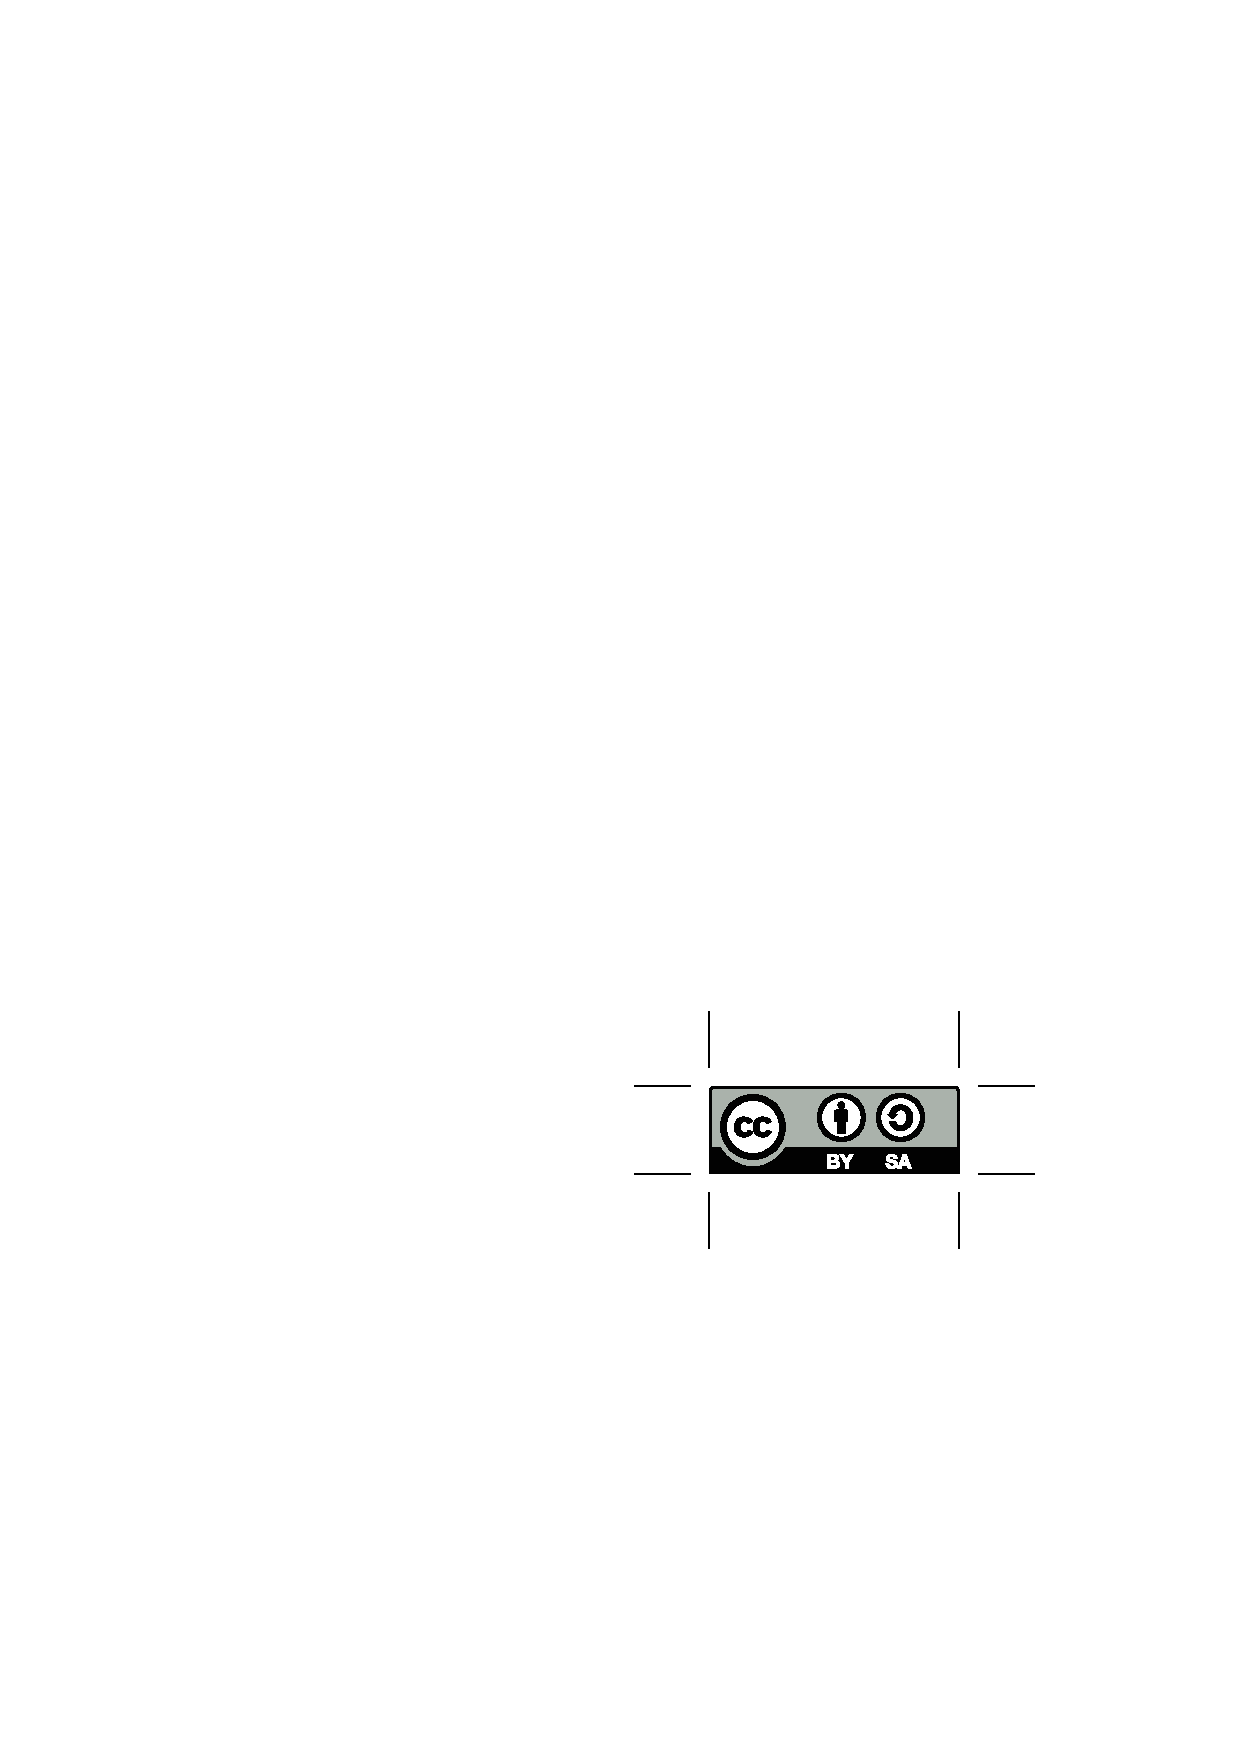
\includegraphics[width=.40\linewidth]{figs/logos/cc/cc_by_sa}}
%        %\\[3em]
%        %\textbf{Illustrations}\\\medskip
%        %\href{http://commons.wikimedia.org/wiki/User:Nojhan}{Johann "nojhan" Dréo} \raisebox{-0.5\height+0.3em}{\href{http://creativecommons.org/licenses/by-sa/2.0/fr/}{
\includegraphics[height=1em]{figs/logos/cc/cc_by_sa_small}}}
%    \end{center}
%\end{frame}
%\note{
%}

